\subsection{\texorpdfstring{$y''+(ax^4+bx^3+cx^2+dx+e)y = 
0$}{y''-(ax4+bx3+cx2+dx+e)y = 0}}

Auch ein Polynom 4-ten Grades stellt kein Problem mehr dar. Die 
Differentialgleichung:

\begin{equation*}
	y''+(ax^4+bx^3+cx^2+dx+e)y = 0
\end{equation*}
ergibt nach dem Einsetzen:

\begin{align*}
	y(x) &= a_0+a_1x-\sum_{k=2}^{\infty} \frac{1}{k(k-1)} (aa_{k-2-4} + 
	ba_{k-2-3} + ca_{k-2-2} + da_{k-2-1} +ea_{k-2-0})x^k
	\\
	&= a_0+a_1x-\sum_{k=2}^{\infty} \frac{1}{k(k-1)} (aa_{k-6} + ba_{k-5} + 
	ca_{k-4} + da_{k-3} +ea_{k-2})x^k, \qquad a_{k<0} = 0
\end{align*}

Auch hier können wir in der Abbildung (\ref{fig:wellen:poly4-dgl}) die 
"Uberg"ange zwischen $\sin$ und $\cos$ bei positiven und $\sinh$ und $\cosh$ 
bei negativen Polynoml"osungen klar erkennen.

\begin{figure}
	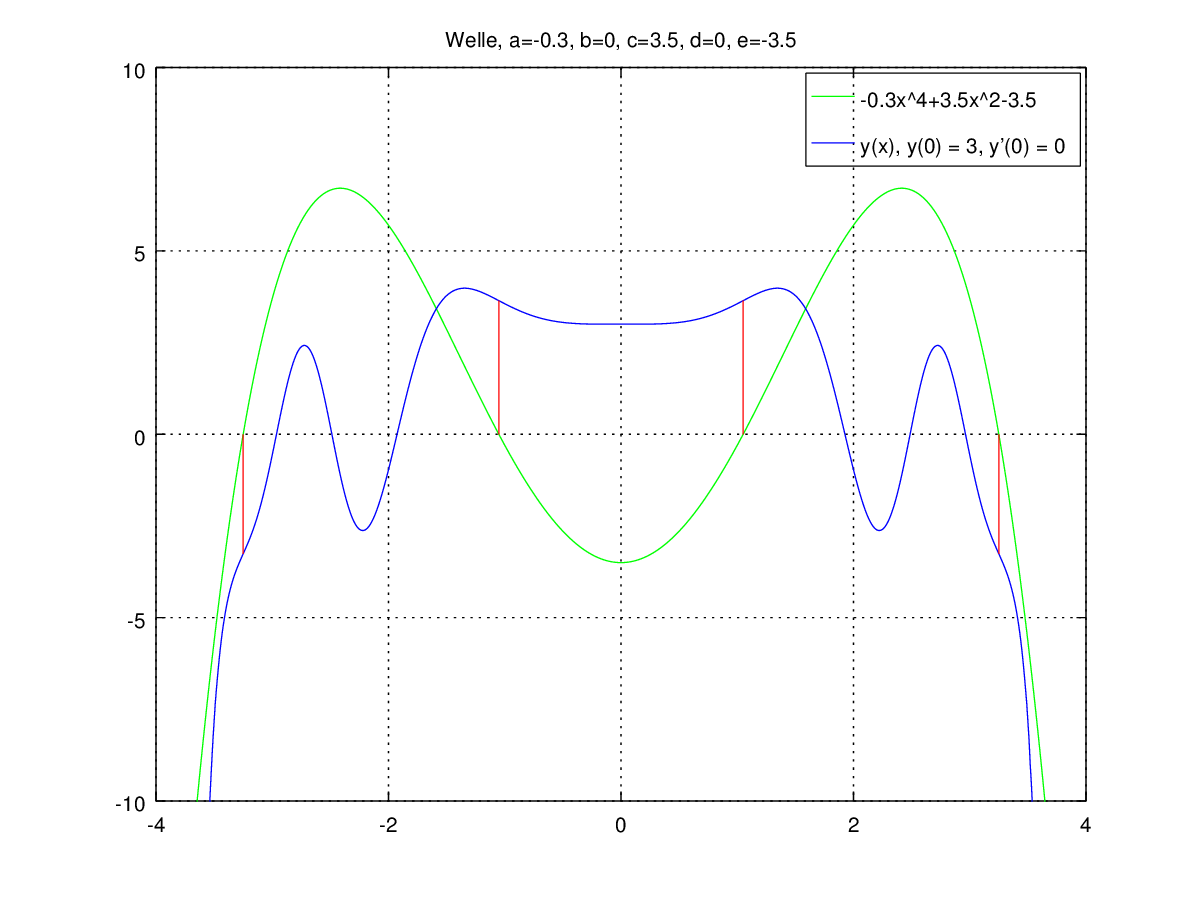
\includegraphics[scale=0.65]{./wellen/images/allgemein/n4.png}
	\caption{L"osung Polynom 4-ten Grades}
	\label{fig:wellen:poly4-dgl}
\end{figure}